%%
%% This is file `sample-sigconf.tex',
%% generated with the docstrip utility.
%%
%% The original source files were:
%%
%% samples.dtx  (with options: `sigconf')
%%
%% IMPORTANT NOTICE:
%%
%% For the copyright see the source file.
%%
%% Any modified versions of this file must be renamed
%% with new filenames distinct from sample-sigconf.tex.
%%
%% For distribution of the original source see the terms
%% for copying and modification in the file samples.dtx.
%%
%% This generated file may be distributed as long as the
%% original source files, as listed above, are part of the
%% same distribution. (The sources need not necessarily be
%% in the same archive or directory.)
%%
%%
%% Commands for TeXCount
%TC:macro \cite [option:text,text]
%TC:macro \citep [option:text,text]
%TC:macro \citet [option:text,text]
%TC:envir table 0 1
%TC:envir table* 0 1
%TC:envir tabular [ignore] word
%TC:envir displaymath 0 word
%TC:envir math 0 word
%TC:envir comment 0 0
%%
%%
%% The first command in your LaTeX source must be the \documentclass command.
\documentclass[sigconf]{acmart}
\usepackage{amsmath}
\usepackage{algorithm}
\usepackage{algorithmic}


%%
%% \BibTeX command to typeset BibTeX logo in the docs
\AtBeginDocument{%
  \providecommand\BibTeX{{%
    \normalfont B\kern-0.5em{\scshape i\kern-0.25em b}\kern-0.8em\TeX}}}

%% Rights management information.  This information is sent to you
%% when you complete the rights form.  These commands have SAMPLE
%% values in them; it is your responsibility as an author to replace
%% the commands and values with those provided to you when you
%% complete the rights form.
\setcopyright{acmcopyright}
\copyrightyear{2022}
\acmYear{2022}
\acmDOI{XXXXXXX.XXXXXXX}

%% These commands are for a PROCEEDINGS abstract or paper.
\acmConference[ISSAC '22]{International Symposium on
Symbolic and Algebraic Computation}{July 04--07,
  2022}{Lille, France}
% \acmPrice{15.00}
% \acmISBN{978-1-4503-XXXX-X/18/06}


%%
%% Submission ID.
%% Use this when submitting an article to a sponsored event. You'll
%% receive a unique submission ID from the organizers
%% of the event, and this ID should be used as the parameter to this command.
%%\acmSubmissionID{123-A56-BU3}

%%
%% The majority of ACM publications use numbered citations and
%% references.  The command \citestyle{authoryear} switches to the
%% "author year" style.
%%
%% If you are preparing content for an event
%% sponsored by ACM SIGGRAPH, you must use the "author year" style of
%% citations and references.
%% Uncommenting
%% the next command will enable that style.
%%\citestyle{acmauthoryear}

%%
%% end of the preamble, start of the body of the document source.
\begin{document}

%%
%% The "title" command has an optional parameter,
%% allowing the author to define a "short title" to be used in page headers.
\title{Root-Squaring for Root-Finding}

%%
%% The "author" command and its associated commands are used to define
%% the authors and their affiliations.
%% Of note is the shared affiliation of the first two authors, and the
%% "authornote" and "authornotemark" commands
%% used to denote shared contribution to the research.
\author{Pedro Soto}
\affiliation{%
    \institution{The Graduate Center, CUNY}
    \city{New York}
    \state{New York}
    \country{USA}
}
\email{psoto@gradcenter.cuny.edu}



\author{Soo Goo}
\affiliation{%
    \institution{The Graduate Center, CUNY}
    \city{New York}
    \state{New York}
    \country{USA}
}
\email{sgo@gradcenter.cuny.edu}
%
% \author{Victor}
% \affiliation{%
%     \institution{CUNY}
%     \city{NY}
%     \state{NY}
%     \country{USA}
% }

% \author{Aparna Patel}
% \affiliation{%
%  \institution{Rajiv Gandhi University}
%  \streetaddress{Rono-Hills}
%  \city{Doimukh}
%  \state{Arunachal Pradesh}
%  \country{India}}
%
% \author{Huifen Chan}
% \affiliation{%
%   \institution{Tsinghua University}
%   \streetaddress{30 Shuangqing Rd}
%   \city{Haidian Qu}
%   \state{Beijing Shi}
%   \country{China}}
%
% \author{Charles Palmer}
% \affiliation{%
%   \institution{Palmer Research Laboratories}
%   \streetaddress{8600 Datapoint Drive}
%   \city{San Antonio}
%   \state{Texas}
%   \country{USA}
%   \postcode{78229}}
% \email{cpalmer@prl.com}
%
% \author{John Smith}
% \affiliation{%
%   \institution{The Th{\o}rv{\"a}ld Group}
%   \streetaddress{1 Th{\o}rv{\"a}ld Circle}
%   \city{Hekla}
%   \country{Iceland}}
% \email{jsmith@affiliation.org}
%
% \author{Julius P. Kumquat}
% \affiliation{%
%   \institution{The Kumquat Consortium}
%   \city{New York}
%   \country{USA}}
% \email{jpkumquat@consortium.net}

%%
%% By default, the full list of authors will be used in the page
%% headers. Often, this list is too long, and will overlap
%% other information printed in the page headers. This command allows
%% the author to define a more concise list
%% of authors' names for this purpose.
\renewcommand{\shortauthors}{Soto and Go, et al.}

%%
%% The abstract is a short summary of the work to be presented in the
%% article.
\begin{abstract}
We revisited the classical root-squaring formula of Dandelin-Lobachevsky-Graeffe for polynomials and found new interesting applications to root-finding.
\end{abstract}

%%
%% The code below is generated by the tool at http://dl.acm.org/ccs.cfm.
%% Please copy and paste the code instead of the example below.
%%
\begin{CCSXML}
<ccs2012>
   <concept>
       <concept_id>10010147.10010148.10010149.10010154</concept_id>
       <concept_desc>Computing methodologies~Hybrid symbolic-numeric methods</concept_desc>
       <concept_significance>500</concept_significance>
       </concept>
 </ccs2012>
\end{CCSXML}

\ccsdesc[500]{Computing methodologies~Hybrid symbolic-numeric methods}



%%
%% Keywords. The author(s) should pick words that accurately describe
%% the work being presented. Separate the keywords with commas.
\keywords{symbolic-numeric computing, root finding, polynomial algorithms, computer algebra}

%% A "teaser" image appears between the author and affiliation
%% information and the body of the document, and typically spans the
%% page.
% \begin{teaserfigure}
%   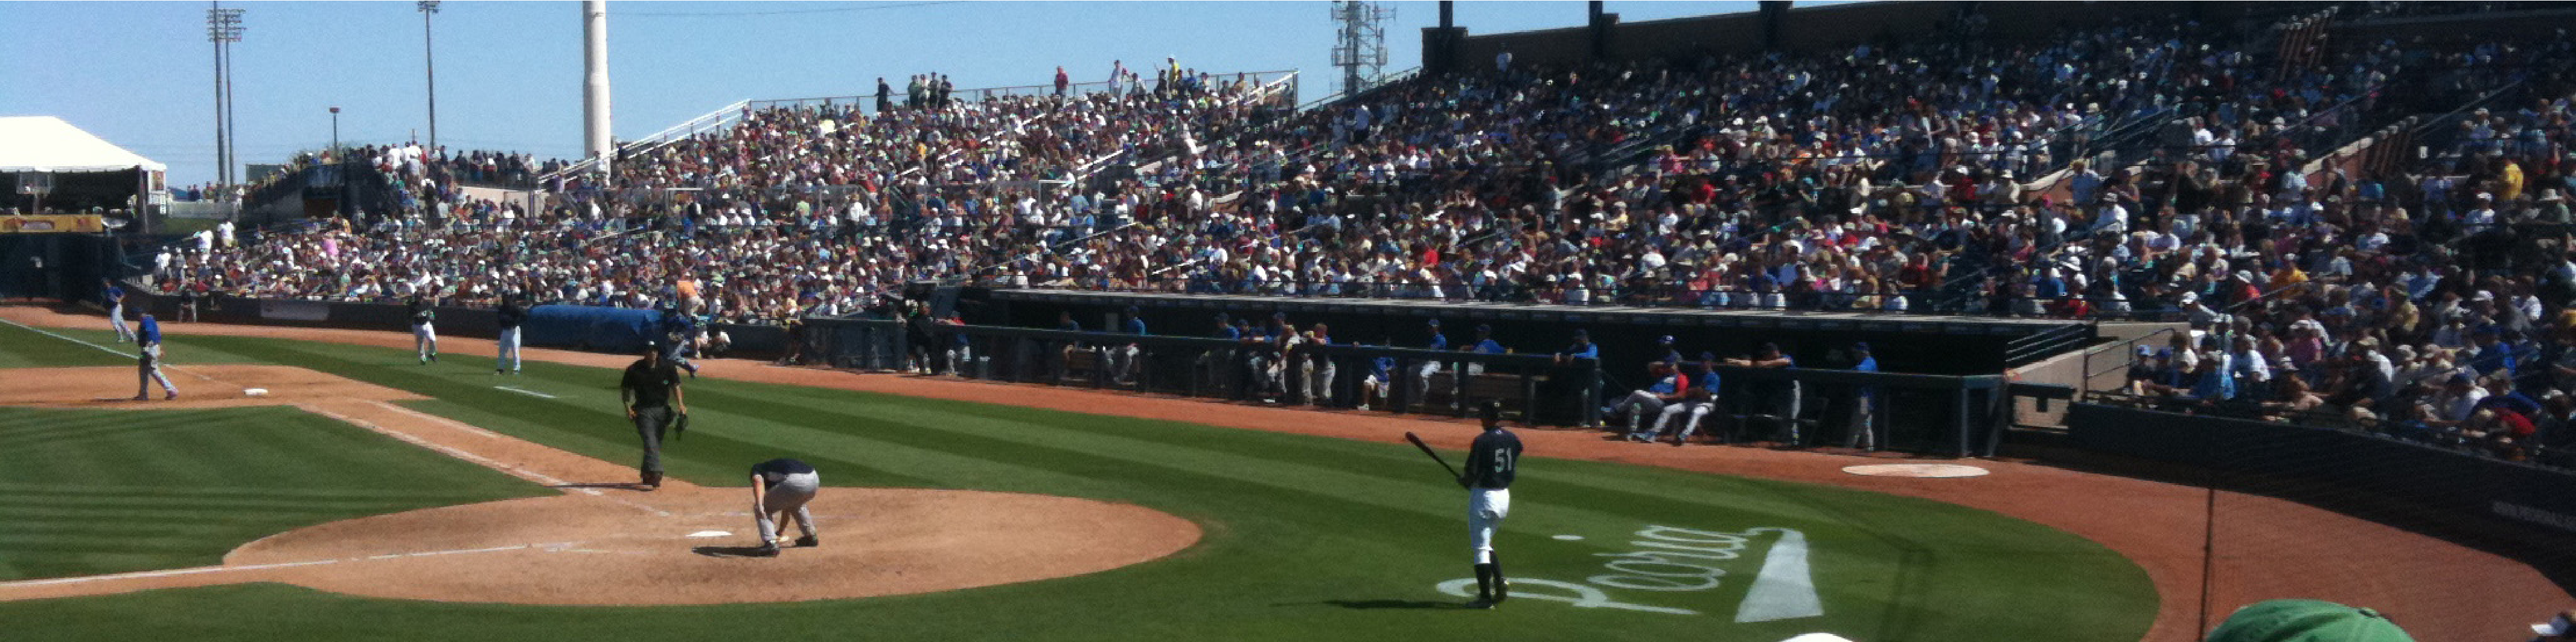
\includegraphics[width=\textwidth]{sampleteaser}
%   \caption{Seattle Mariners at Spring Training, 2010.}
%   \Description{Enjoying the baseball game from the third-base
%   seats. Ichiro Suzuki preparing to bat.}
%   \label{fig:teaser}
% \end{teaserfigure}

%%
%% This command processes the author and affiliation and title
%% information and builds the first part of the formatted document.
\maketitle

\section{Introduction}


\section{Related Works}

\section{Background}

\section{Motivating Example}

\begin{figure}[h]
  \centering
  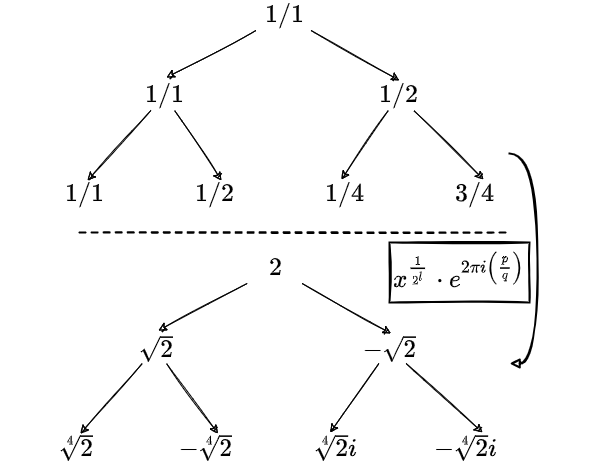
\includegraphics[width=\linewidth]{rational_root_tree.png}
  \caption{The upper tree depicts the steps of \textsc{\textsc{Circle\_Roots\_Rational\_Form}}(p,q,l) in Alg.\ref{alg:circ_roots_rational_form} for $l=2$, $p=1$, and $q=1$. The lower tree depicts the steps of \textsc{Roots}($r,t,u,l$) in Alg.\ref{alg:roots} for $r=2$, $l=2$, $p=1$, and $q=1$}
  \Description{}
\end{figure}

\begin{figure}[h]
  \centering
  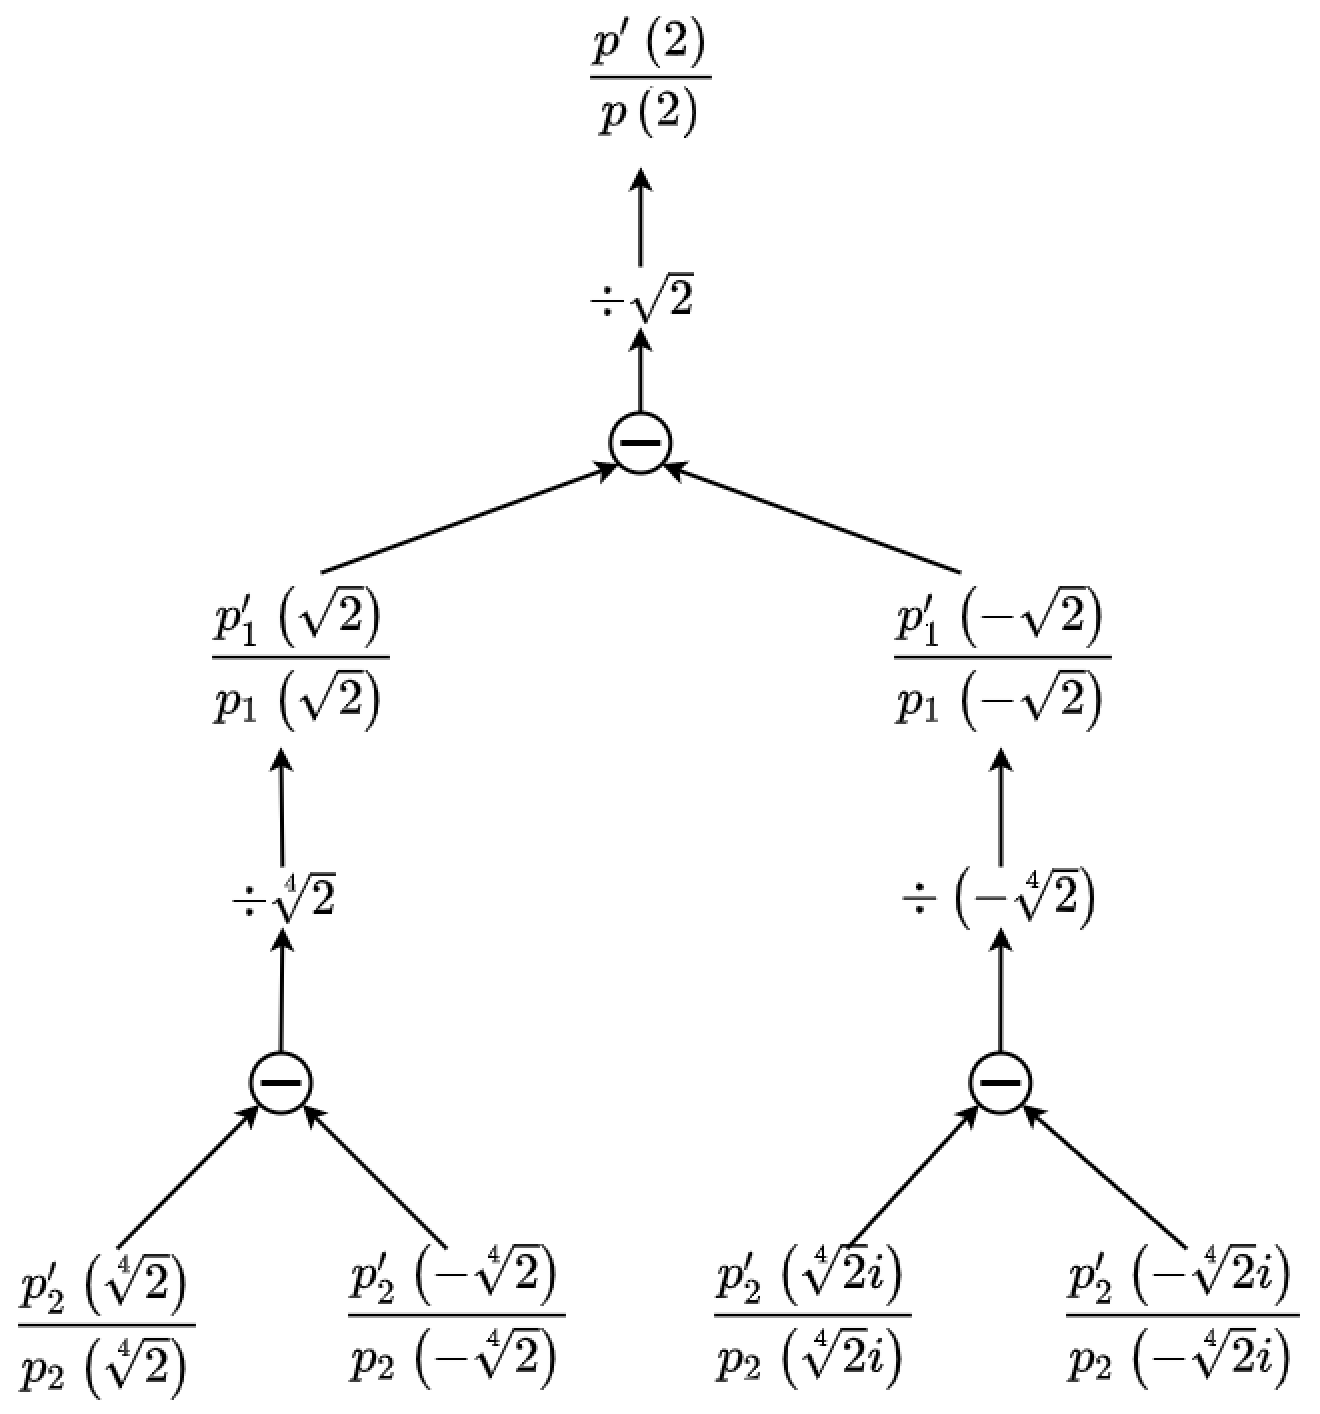
\includegraphics[width=\linewidth]{p_prime.png}
  \caption{The steps of \textsc{DLG\_Rational\_Rorm}($p,p^\prime,r,t,u,l$) in Alg.\ref{alg:DLG_rational_form} for $r=2$, $l=2$, $t=1$, and $u=1$.}
  \Description{}
\end{figure}



\section{Algorithm Design}


\begin{algorithm}
   \caption{\textsc{Circle\_Roots\_Rational\_Form}($p,q,l$)}
   \label{alg:circ_roots_rational_form}
\begin{algorithmic}
\IF{ $p\%q$ == 0}
  \STATE  $r, s$ := (1,1)
\ELSE
  \STATE  $r, s$ := ($p$,$2q$)
\ENDIF
  \IF{ r\%s == 0}
    \STATE $t, u$ := (1,2)
  \ELSE
    \STATE $t, u$ := $(2r+s, 2s)$
  \ENDIF
	  \IF{$l$ == 1}
		  \RETURN [($r,s$),($t,u$)]
	\ELSIF {$l$ != 0}
		\STATE left  := \textsc{Circle\_Roots\_Rational\_Form}($r,s,l-1$)
		\STATE right := \textsc{Circle\_Roots\_Rational\_Form}($t,u,l-1$)
		\RETURN left $\cup$ right
	\ELSE
		\RETURN  [($p,q$)]
      \ENDIF
\end{algorithmic}
\end{algorithm}

\begin{algorithm}
\caption{\textsc{Roots}($r,t,u,l$)}
\label{alg:roots}
\begin{algorithmic}
\STATE root\_tree = \textsc{Circle\_Roots\_Rational\_Form}($p,q,l$)
\STATE circ\_root = [$\exp\left(2\cdot\pi\cdot i \cdot \frac{r}{s}\right)$ for $r,s$ in root\_tree]
% \STATE circ\_root       = circ\_roots($t,u,l$)
\STATE roots =[$\sqrt[2^l]{r}\cdot$root for root in circ\_root]
\end{algorithmic}
\end{algorithm}


% \begin{algorithm}
%    \caption{circ\_roots\_rational\_form($p,q,l$)}
%    \label{alg:circ_roots_rational_form}
% \begin{algorithmic}
%   \STATE $r, s$  := angle\_sq\_root($p,q$)
% 	\STATE $t, u$  := angle\_neg($r,s$)
% 	  \IF{$l$ == 1}
% 		  \RETURN [($r,s$),($t,u$)]
% 	\ELSIF {$l$ != 0}
% 		\STATE left  := circ\_roots\_rational\_form($r,s,l-1$)
% 		\STATE right := circ\_roots\_rational\_form($t,u,l-1$)
% 		\RETURN left $\cup$ right
% 	\ELSE
% 		\RETURN  [($p,q$)]
%       \ENDIF
% \end{algorithmic}
% \end{algorithm}


% \begin{algorithm}
% \caption{angle\_sq\_root(p,q)}
% \label{alg:angle_sq_root}
% \begin{algorithmic}
% 	\IF{ $p\%q$ == 0}
% 		\RETURN  (1,1)
% 	\ELSE
% 		\RETURN  ($p$,$2q$)
%   \ENDIF
% \end{algorithmic}
% \end{algorithm}
%
%
% \begin{algorithm}
% \caption{angle\_neg(p,q)}
% \label{alg:angle_neg}
% \begin{algorithmic}
% 	\IF{ p\%q == 0}
% 		\RETURN  (1,2)
% 	\ELSE
% 		\RETURN  $(2p+q, 2q)$
%   \ENDIF
% \end{algorithmic}
% \end{algorithm}




% \begin{algorithm}
% \caption{circ\_roots($p,q,l$):}
% \label{alg:circ_roots}
% \begin{algorithmic}
% \STATE roots = circ\_roots\_rational\_form($p,q,l$)
% \RETURN [$\exp\left(2\cdot\pi\cdot i \cdot \frac{r}{s}\right)$ for r,s in roots]
% \end{algorithmic}
% \end{algorithm}





% \clearpage

\begin{algorithm}
\caption{\textsc{DLG\_Rational\_Form}($p,p^\prime,r,t,u,l$)}
\label{alg:DLG_rational_form}
\begin{algorithmic}
\STATE 	root      := \textsc{Roots}($r,t,u,l$)
\FOR {$r_i \in $ root}
\STATE 	base\_step[$i$] := $\frac{p^\prime(r_i)}{p(r_i)}$
\ENDFOR
\STATE  diff[0]   := base\_step
\FOR {$i \leq l$}
\FOR {$j \leq 2^{l-i-1}$}
\STATE 			diff[$i+1$][$j$]:=$\frac{1}{2}\frac{\text{diff}[i][2j]-\text{diff}[i][2j+1]}{\text{root}[2j]}$
\STATE 		root = roots($r,t,u,l-1-i$)
\ENDFOR
\ENDFOR
\RETURN derivs$[l][0]$
\end{algorithmic}
\end{algorithm}





\begin{algorithm}
\caption{\textsc{DLG}($p,p^\prime,l,x, \epsilon$)}
\label{alg:rational_angle_approx}
\begin{algorithmic}
\STATE angle     := $\frac{1}{2\pi i} \log (x)$
\STATE Set $t, u$      := angle\_as\_integer\_ratio(angle, $\epsilon$)
\STATE $r$      := $|x|$
\RETURN \textsc{DLG\_Rational\_Rorm}($p,p^\prime,r,t,u,l$)
\end{algorithmic}
\end{algorithm}



% def DLG_rational_form(p,dp,r,t,u,l):
% 	root       = roots(r,t,u,l)
% 	base_step  = [dp(r)*np.reciprocal(p(r)) for r in root]
% 	derivs     = [base_step]
% 	for i in range(l):
% 		derivs.append([])
% 		for j in range(2**(l-i-1)):
% 			derivs[i+1].append((np.reciprocal(root[2*j])/2)*(derivs[i][2*j] - derivs[i][2*j+1]))
% 		root = roots(r,t,u,l-1-i)
% 	return derivs[l][0]





\section{Theoretical Analysis}
% \newpage
% \clearpage
\section{Experimental Results}

% \begin{figure}[h]
%   \centering
%   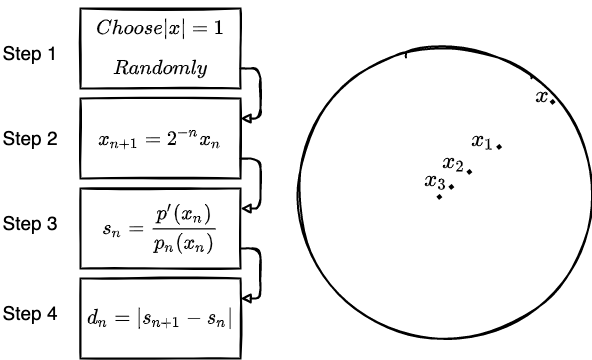
\includegraphics[width=\linewidth]{limit_test.png}
%   \caption{Limit test.}
%   \Description{The procedure for taking the limit to zero.}
% \end{figure}


\section{Conclusion}

%%
%% The acknowledgments section is defined using the "acks" environment
%% (and NOT an unnumbered section). This ensures the proper
%% identification of the section in the article metadata, and the
%% consistent spelling of the heading.
% \begin{acks}
% To Robert, for the bagels and explaining CMYK and color spaces.
% \end{acks}

%%
%% The next two lines define the bibliography style to be used, and
%% the bibliography file.
\bibliographystyle{ACM-Reference-Format}
\bibliography{sample-base}

%%
%% If your work has an appendix, this is the place to put it.
\appendix



\end{document}
\endinput
%%
%% End of file `sample-sigconf.tex'.
